\section{仿生机器鼠动作规划}
行为(Behaviour)是指由个体、器官、系统或者人造物做出的一系列动作序列,这些动作往往是对自身或者包含自身和其他个体、器官或者系统的物理环境的反应\cite{mintonBeliefSystemsReligion2013}。尽管在生物学中,科学家对如何精确定义行为仍然存在分歧,但一种常见解释为,行为是包含其全部器官的内部协调反应,而这种反应是对其内部或外部刺激做出的\cite{levitisBehaviouralBiologistsNot2009}。由此可见,行为应当是一系列动作的有意义组合,这一“意义”应当是其目标的完成情况。对生物鼠而言,其行为应当是以引起其交互对象适当反应为目的,而开展行为交互实验的机器鼠也应当遵守这一准则。

一直以来,研究者们对生物鼠行为做了较为丰富、详细的研究。统计表明,生物鼠不同行为出现的频率存在较大差异。当两只生物鼠处于同意环境中时,仍然会产生大量不具有交互意义的行为,以时间度量,这些非交互性的行为占到所有行为的$60\%$左右\cite{ISI:000436213800018},同时那些交互性的行为所占时间比例也不同。

虽然生物鼠的行为受到多种因素影响,例如食物、水源等,但在行为交互实验中对生物鼠行为影响最为显著的因素为其交互伙伴的相关属性,这些属性包括其气味、性别、年龄等实验中的不变特性,也包括其动作、叫声等在实验过程中经常变化的特性\cite{whishawBehaviorLaboratoryRat2005}。\citeauthor{BarnettSTheRat}对生物鼠的行为进行的研究表明,当两只生物鼠交互时,它们将倾向于表现征服、服从、梳理和嗅探四种行为模式,这四种模式具有一定的个体对称性,例如,当其中一只生物鼠处于征服状态时,另一只生物鼠通常表现为服从状态\cite{BarnettSTheRat}。而当两只生物鼠处于未交互状态时,其表现行为包括探索、直立等个体行为。
% \begin{figure}[htbp]
%   %\vspace{13pt}
%   \centering
%   \subfigure[征服与服从]{\label{figure_crandwal}
%   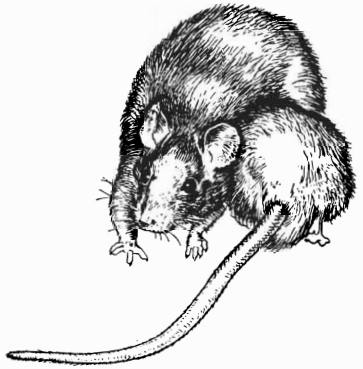
\includegraphics[height=0.24\linewidth]{images/ch02/crawlandwalk.png}
%   }
%   \subfigure[梳理]{\label{figure_grooming}
%   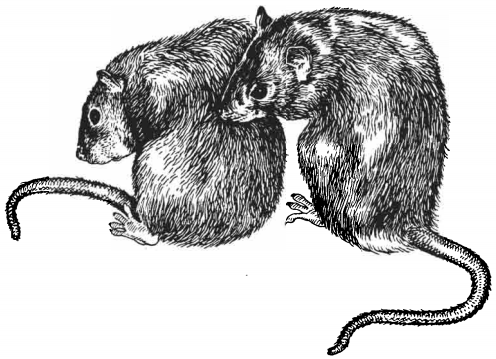
\includegraphics[height=0.24\linewidth]{images/ch02/groom.png}
%   }
%   \subfigure[嗅探]{\label{figure_sniff}
%   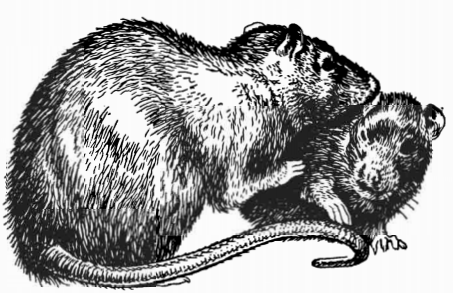
\includegraphics[height=0.24\linewidth]{images/ch02/sniff.png}
%   }
%   \caption{两只生物鼠主要交互行为\cite{BarnettSTheRat}}\label{figure_2ratbehav}
% \end{figure}

根据上述分析,对仿生机器鼠的动作设计应当遵循相似性、紧密性和典型性的原则,对相应各选取原则的解释如下。
\begin{enumerate}[leftmargin=0em, listparindent=2em, parsep=0em, topsep=0em, label=(\theenumi)]
%\setlength{\leftmargin}{0em}
\setlength{\itemindent}{4em}
\setlength{\labelsep}{0em}
\setlength{\labelwidth}{2em}
\setlength{\parsep}{0em}
\setlength{\itemsep}{0em}
\setlength{\topsep}{0em}
%\setlength{\listparindent}{2em}
  \item 与生物鼠相应动作具有相似性。
  \item 与交互紧密相关。
  \item 具有典型性。
\end{enumerate}

根据上述原则,本文选定直行、后退、左转、右转、直立、嗅探、梳理、被梳理、匍匐和攀爬10种动作作为仿生机器鼠的基本动作。
% \begin{enumerate}[leftmargin=0em, listparindent=2em, parsep=0em, topsep=0em, label=(\theenumi)]
% %\setlength{\leftmargin}{0em}
% \setlength{\itemindent}{4em}
% \setlength{\labelsep}{0em}
% \setlength{\labelwidth}{2em}
% \setlength{\parsep}{0em}
% \setlength{\itemsep}{0em}
% \setlength{\topsep}{0em}
% %\setlength{\listparindent}{2em}
%   \item 直行是生物鼠在实验环境中出现频率最高的动作,这是由于无论受到何种刺激,生物鼠总有躲避或者靠近的倾向,而生物鼠与其伙伴进行交互也离不开大量的位置变化。例如,生物鼠表现接近(Approaching)行为时,总是从距离较远的地方向其交互伙伴移动,其轨迹通常是直线(图\ref{figure_appr})。

%       这一动作的实现方式较为简单。由于机器鼠采用两轮差速驱动方式,因此只需控制两轮转速一致,并且与生物鼠运动速度相同,即可在理论上使得仿生机器鼠沿直线行走,但应注意摩擦力等外部因素的影响使得这一方式存在偏差,引入其角速度作为反馈可以解决这一问题。
% \begin{figure}[htbp]
%   %\vspace{13pt}
%   \centering
%   \subfigure[$t_0$]{\label{figure_appr_0000}
%   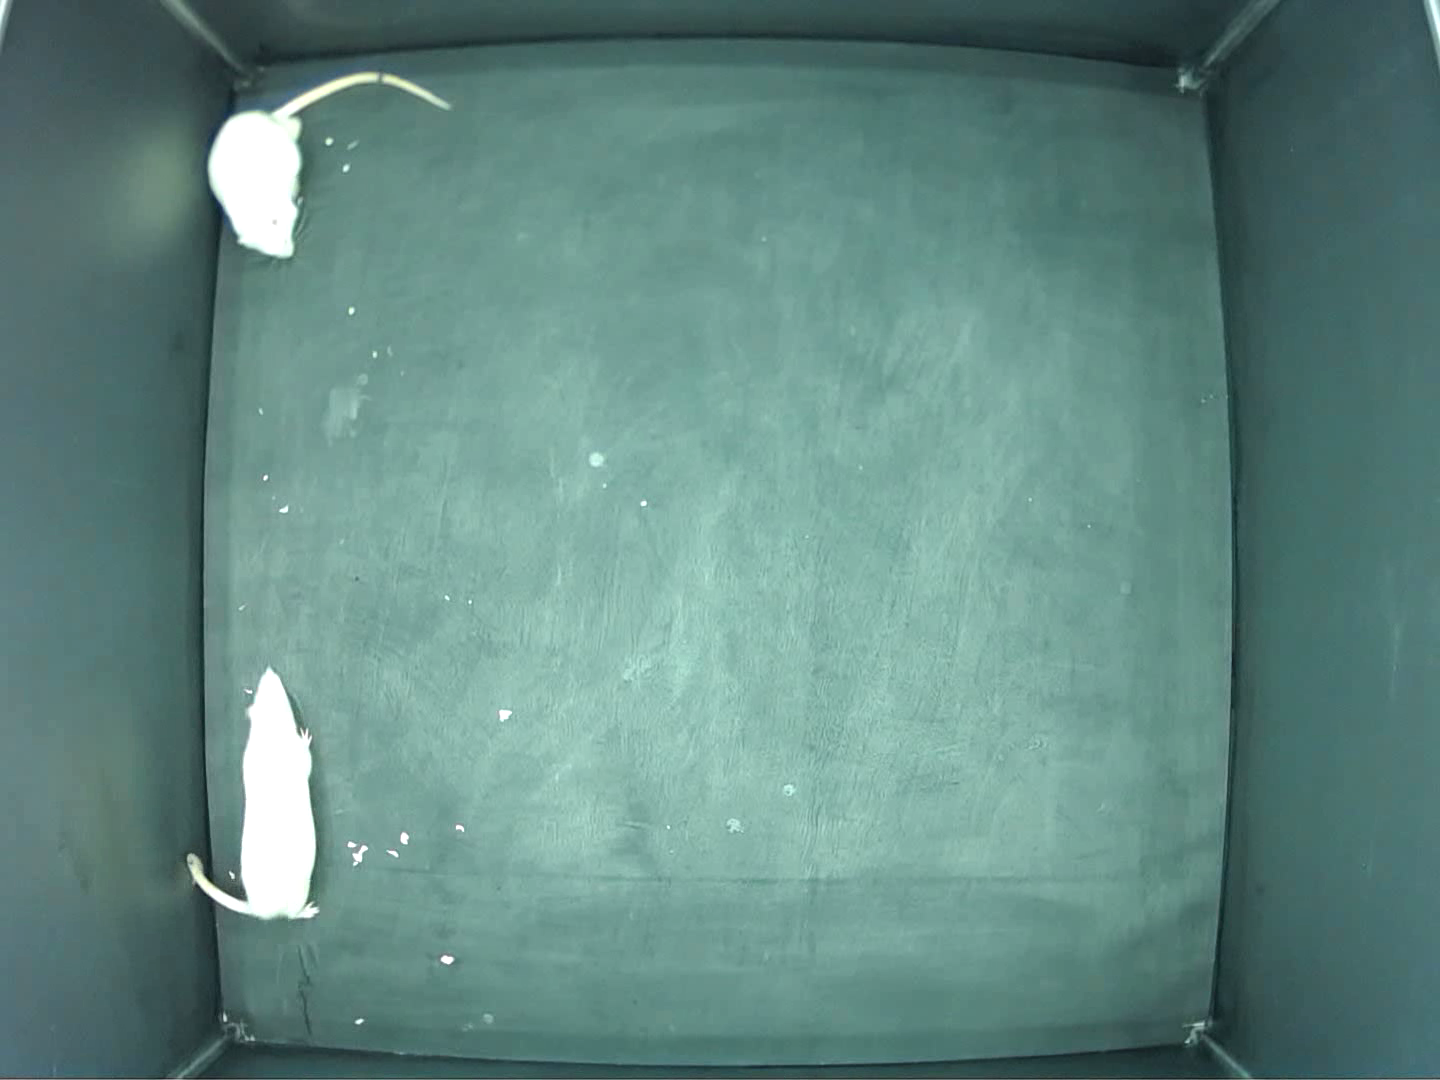
\includegraphics[width=0.27\linewidth]{images/ch02/action/appr/0000.png}
%   }
%   \subfigure[$t_0+432~ms$]{\label{figure_appr_0432}
%   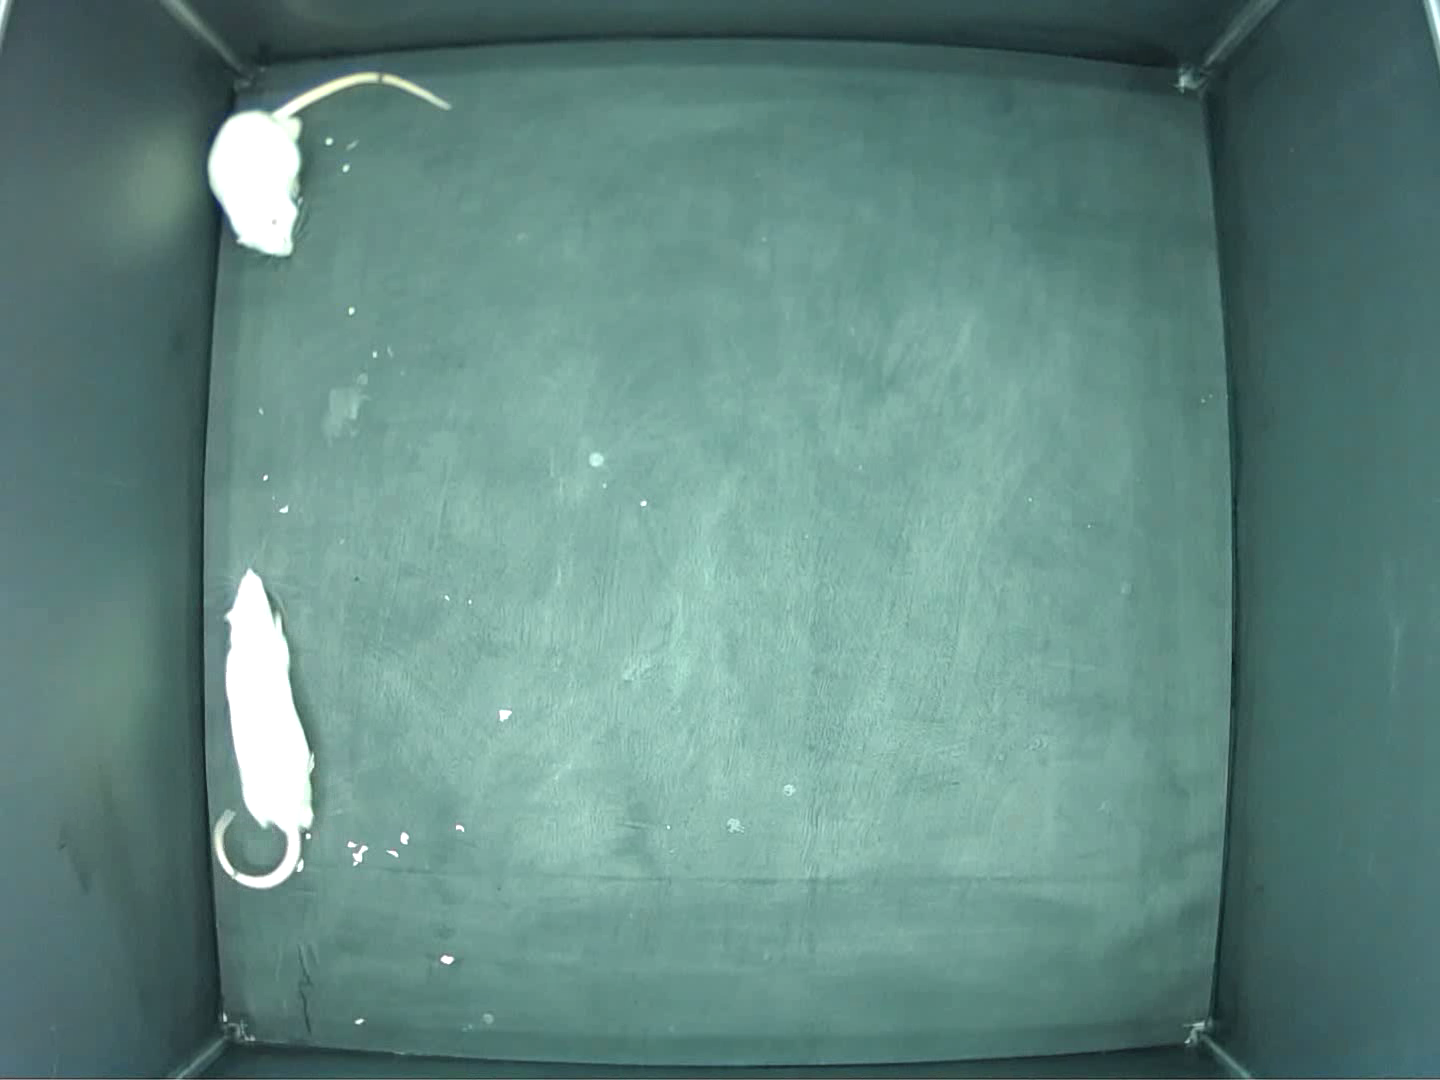
\includegraphics[width=0.27\linewidth]{images/ch02/action/appr/0432.png}
%   }
%   \subfigure[$t_0+948~ms$]{\label{figure_appr_0948}
%   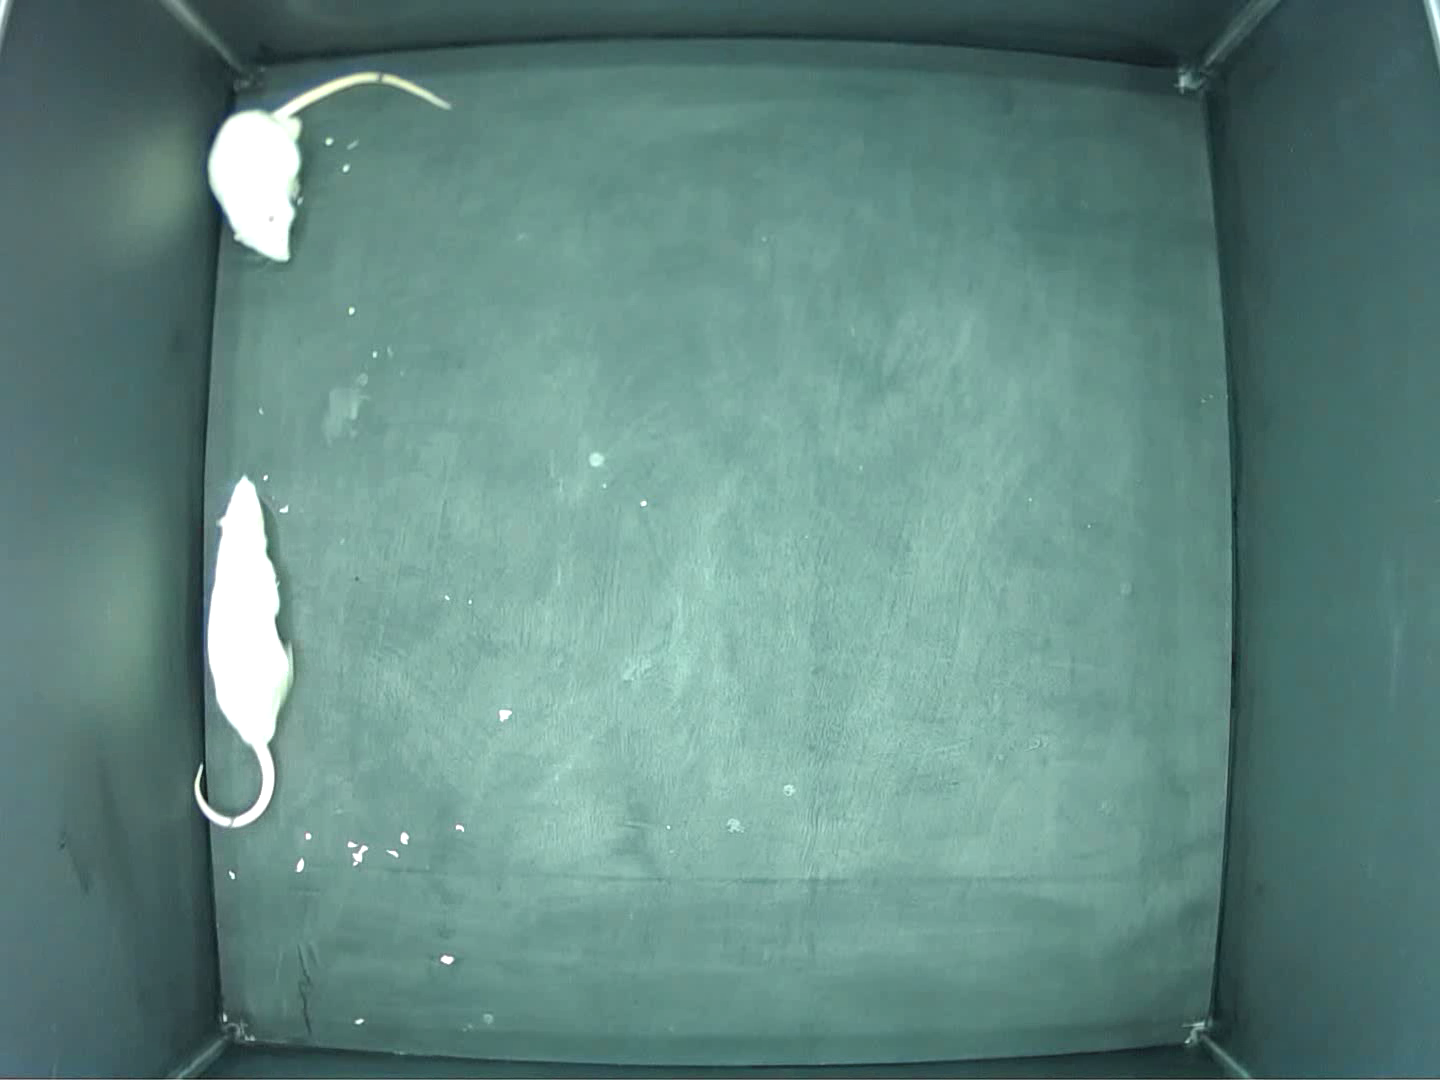
\includegraphics[width=0.27\linewidth]{images/ch02/action/appr/0948.png}
%   }\\
%   \subfigure[$t_0+1535~ms$]{\label{figure_appr_1535}
%   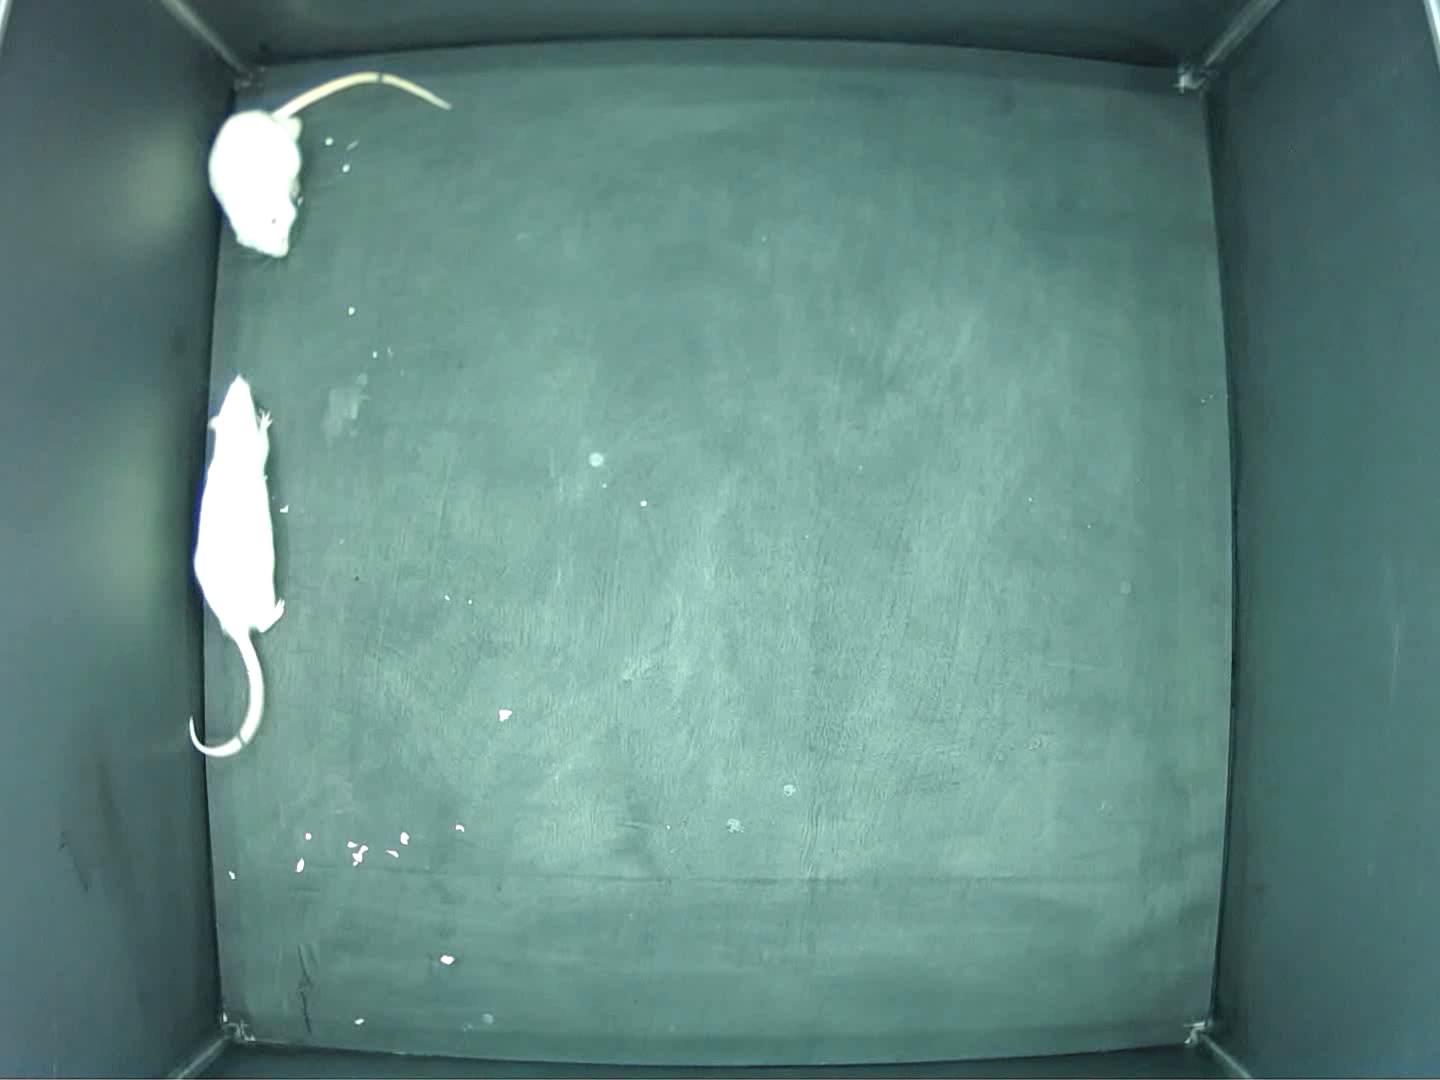
\includegraphics[width=0.27\linewidth]{images/ch02/action/appr/1535.png}
%   }
%   \subfigure[$t_0+2007~ms$]{\label{figure_appr_2007}
%   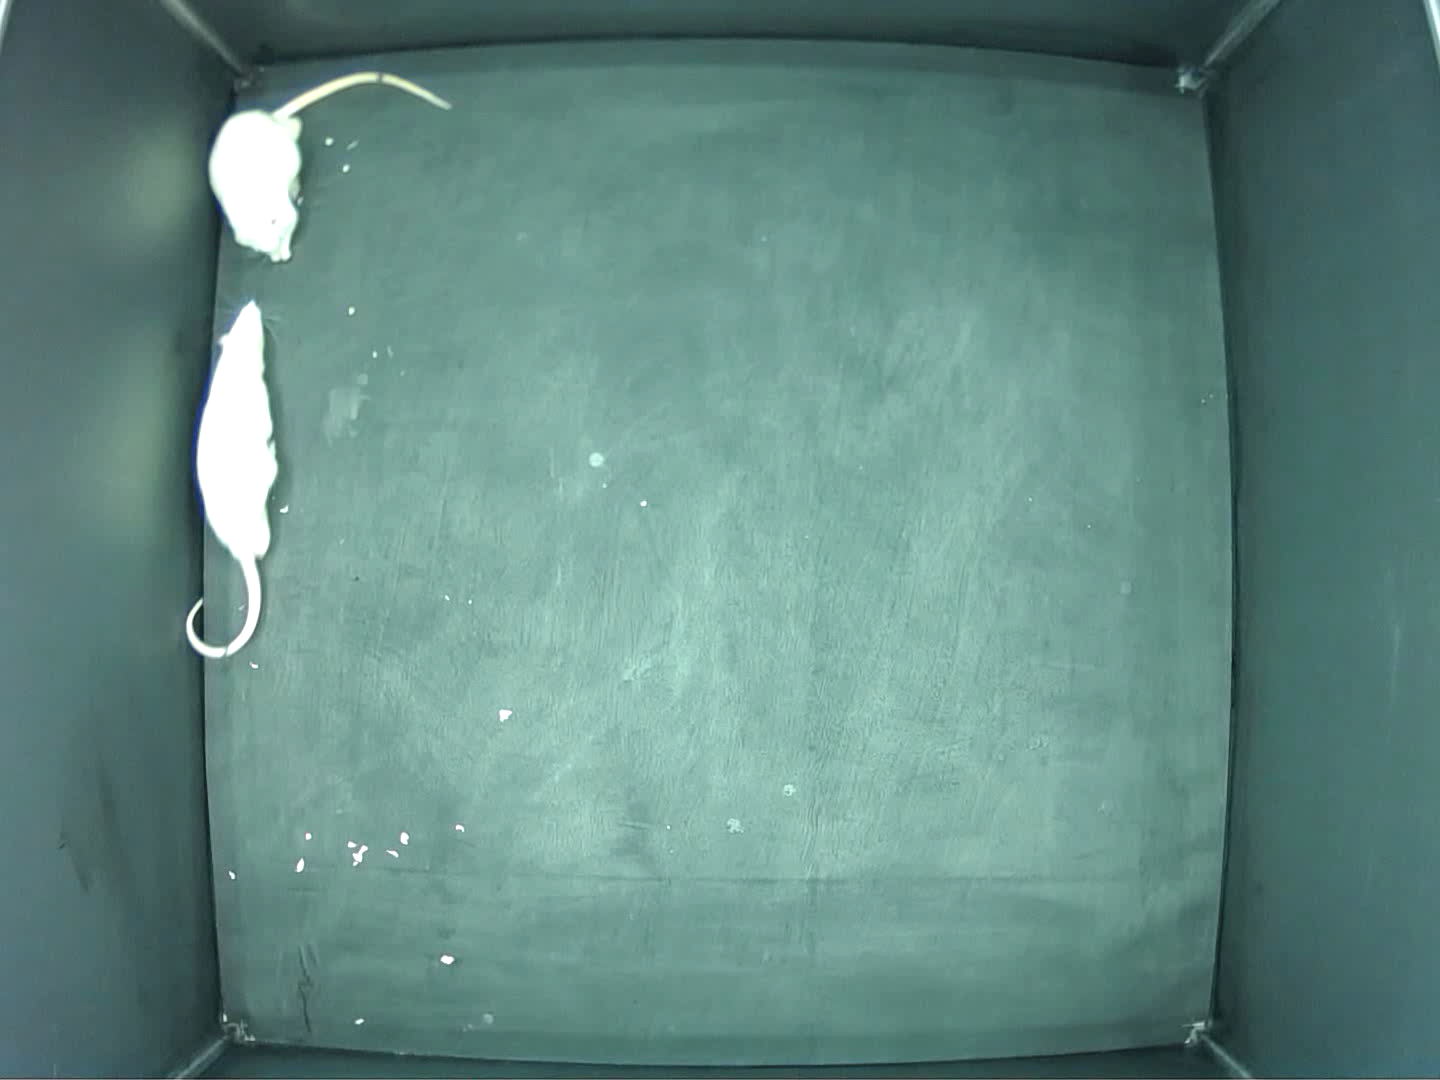
\includegraphics[width=0.27\linewidth]{images/ch02/action/appr/2007.png}
%   }
%   \subfigure[$t_0+2541~ms$]{\label{figure_appr_2541}
%   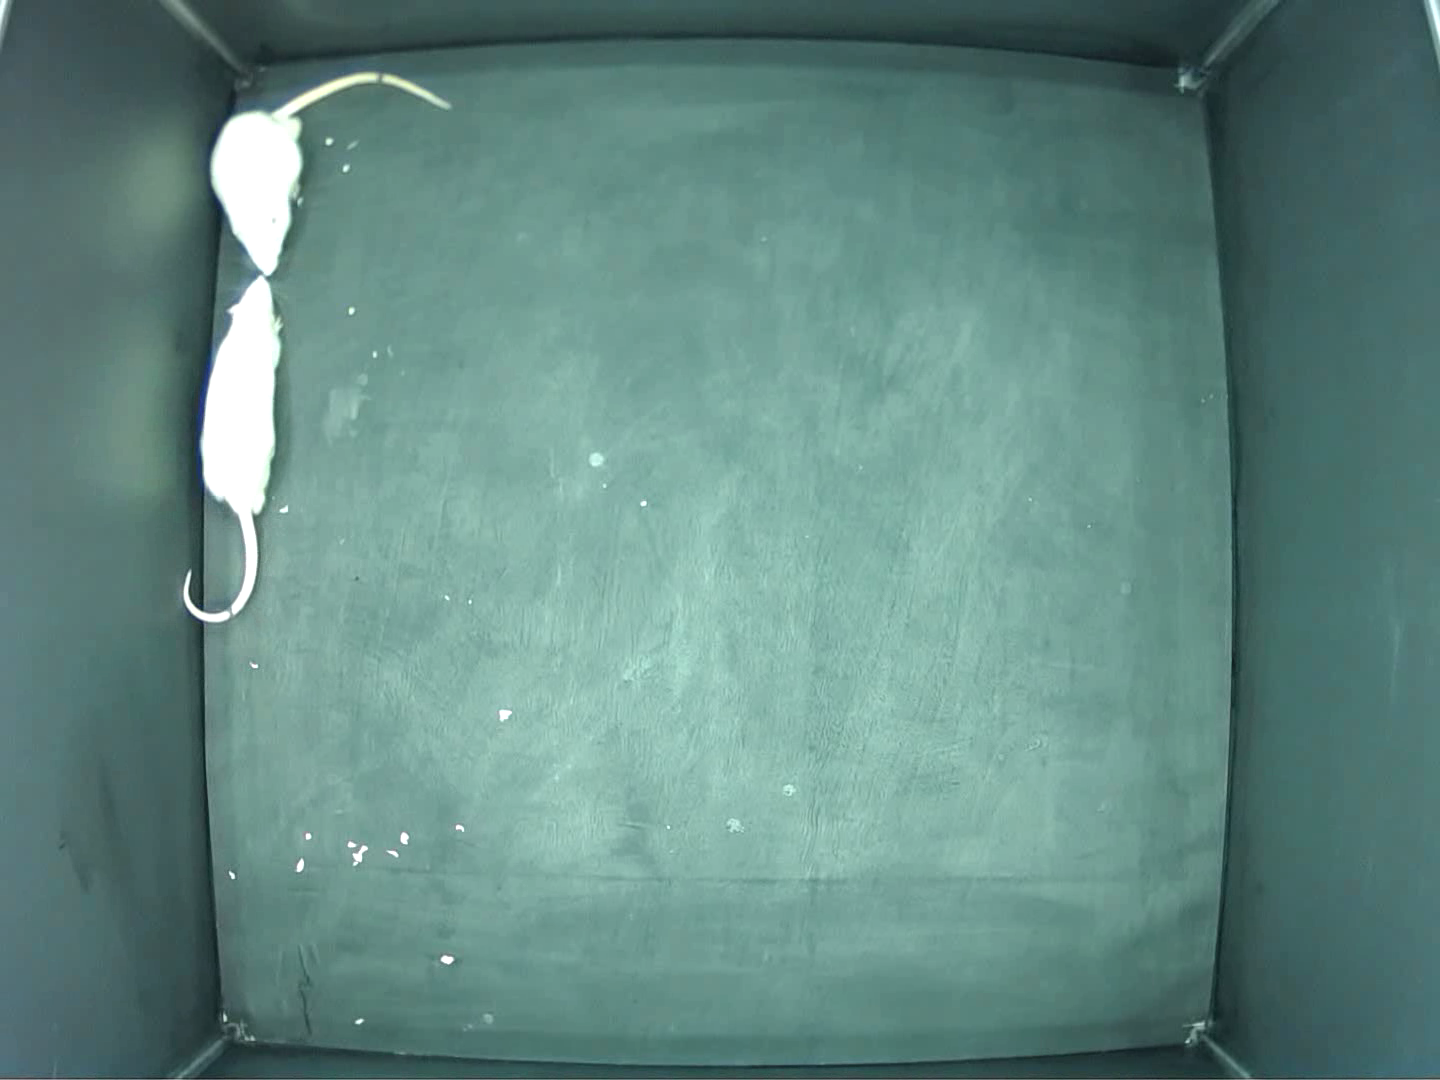
\includegraphics[width=0.27\linewidth]{images/ch02/action/appr/2541.png}
%   }
%   \caption{实验环境中生物鼠接近其交互伙伴}\label{figure_appr}
% \end{figure}

%   \item 后退并非生物鼠的高频率动作,但对仿生机器鼠的运动意义重大。限于仿生机器鼠结构仍然存在一定的缺陷,在运动时存在机器鼠被障碍(物体、生物鼠或者另一机器鼠)困住的可能,尽管这一情况出现的概率较低,但保留后退这一基本行为可以保证其在被困时迅速脱离,保证实验的延续。

%       后退的实现与前进相似。
%   \item 左转(图\ref{figure_turn})和右转是生物鼠的常见动作,这与前进相似。生物鼠在直线前进一定距离后,总有改变其运动方向的需要:既有可能躲避前方的障碍,也有可能受到交互对象的吸引。观察表明生物鼠转向时主要依靠腰部和前肢的运动,由于后肢参与程度较低,转向后总是停留在原处。

%       实现机器鼠的转向依靠左、右轮运动方向的差异实现。
% \begin{figure}[htbp]
%   %\vspace{13pt}
%   \centering
%   \subfigure[$t_0$]{\label{figure_turn_0000}
%   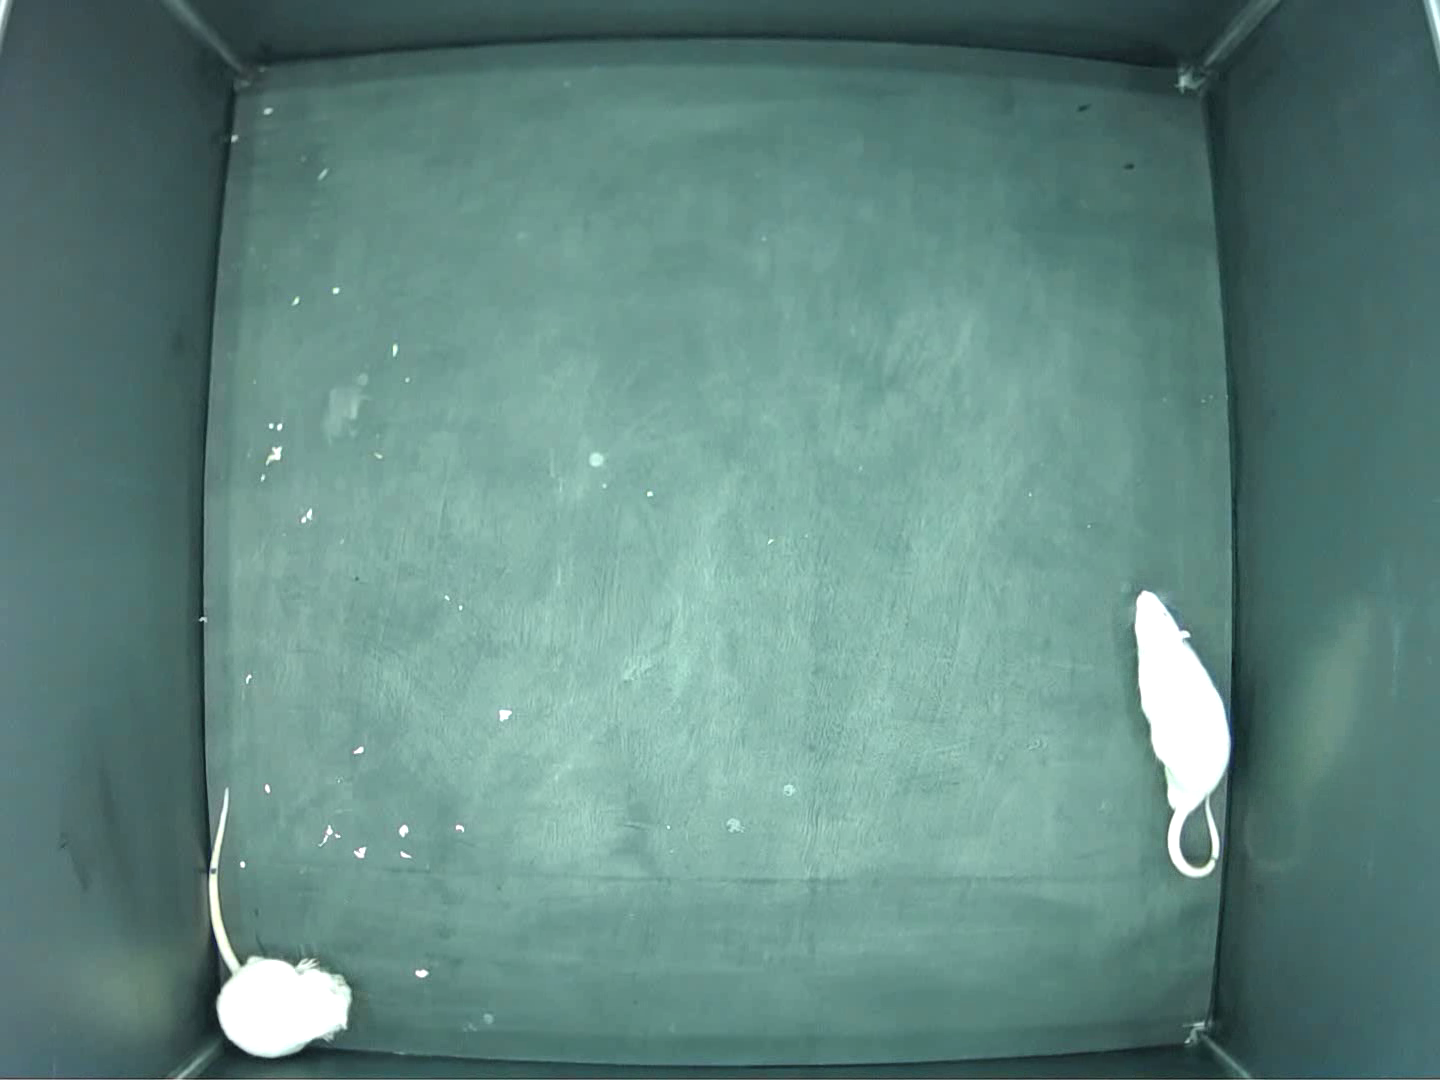
\includegraphics[width=0.27\linewidth]{images/ch02/action/turn/0000.png}
%   }
%   \subfigure[$t_0+430~ms$]{\label{figure_turn_0330}
%   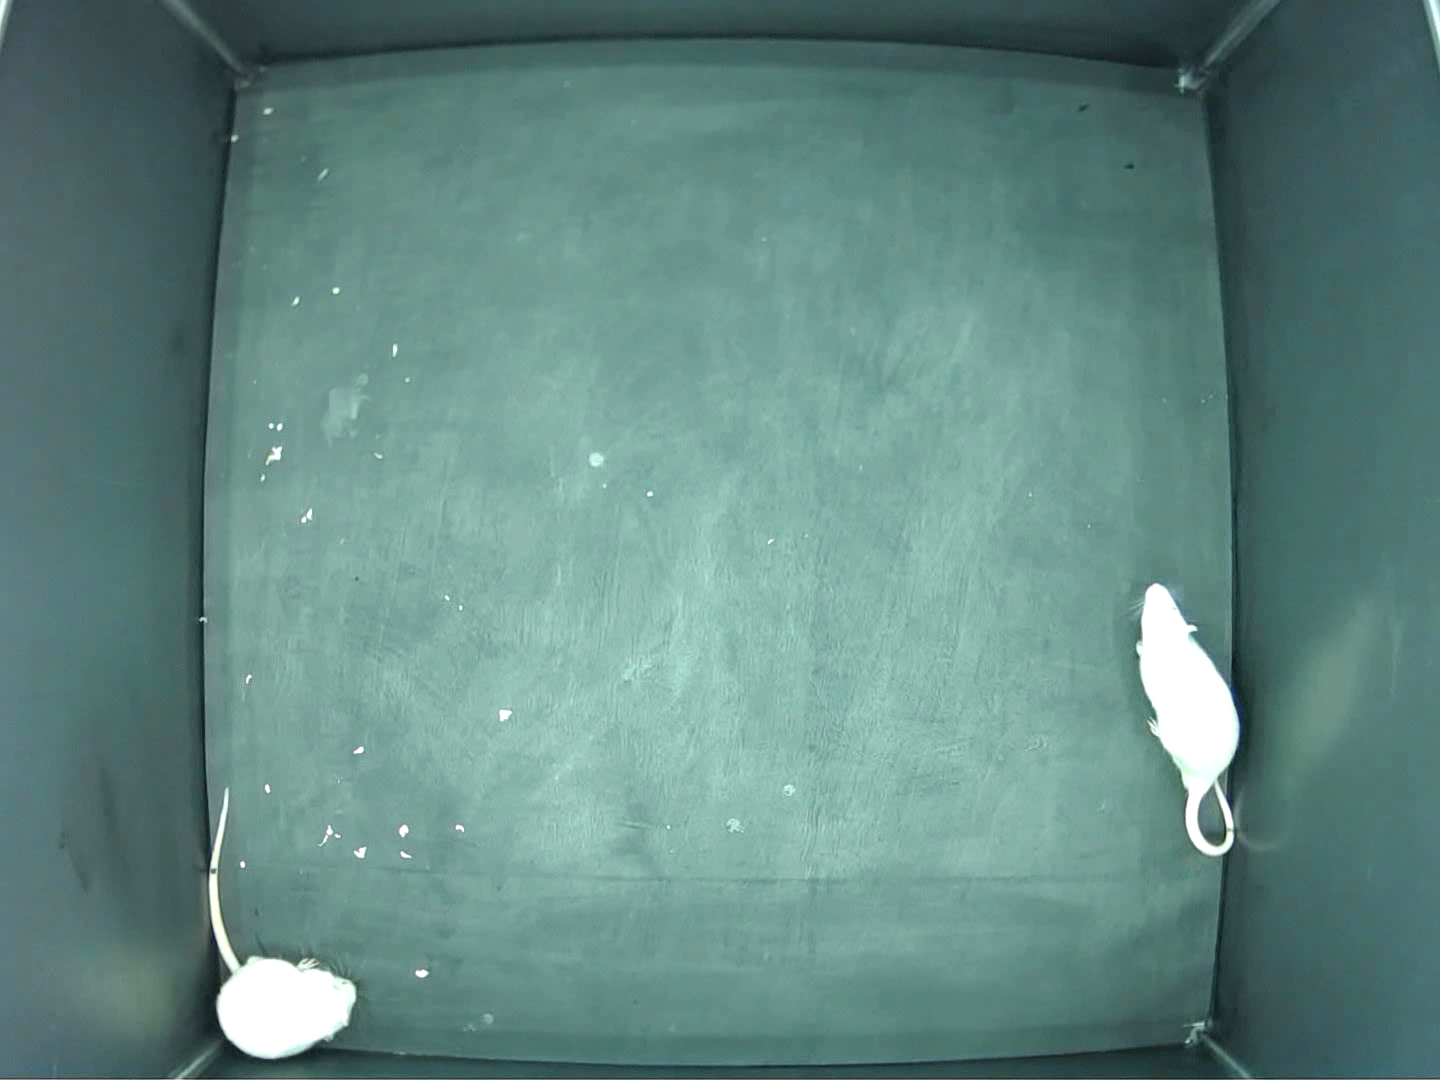
\includegraphics[width=0.27\linewidth]{images/ch02/action/turn/0330.png}
%   }
%   \subfigure[$t_0+1050~ms$]{\label{figure_turn_0650}
%   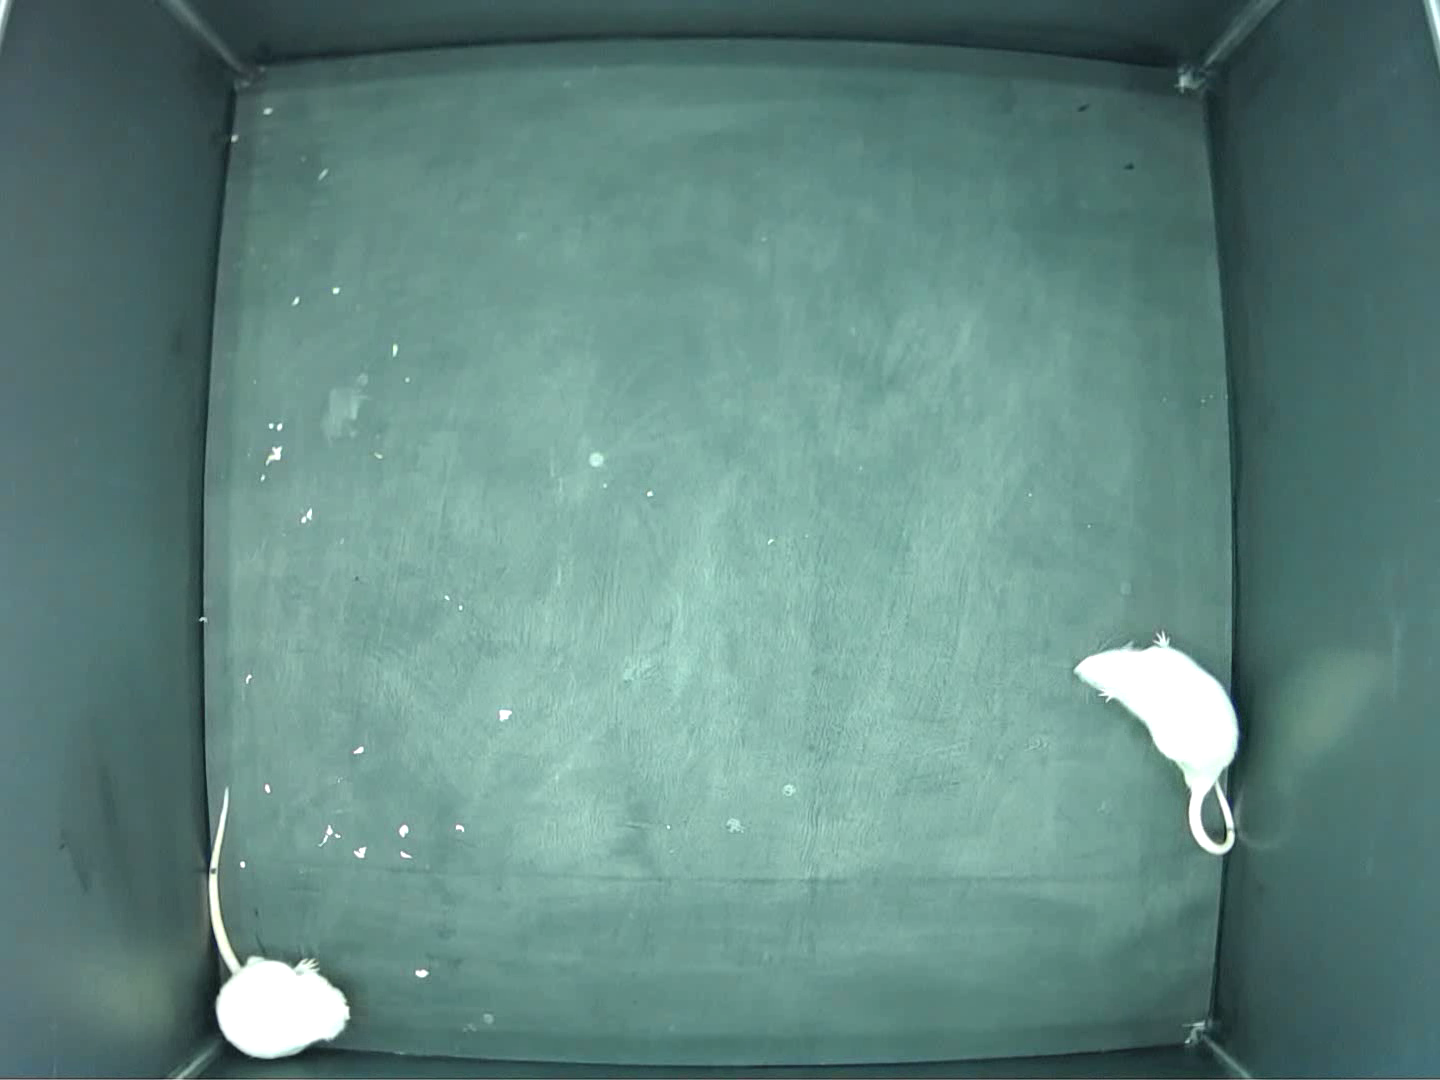
\includegraphics[width=0.27\linewidth]{images/ch02/action/turn/0650.png}
%   }\\
%   \subfigure[$t_0+1699~ms$]{\label{figure_turn_0964}
%   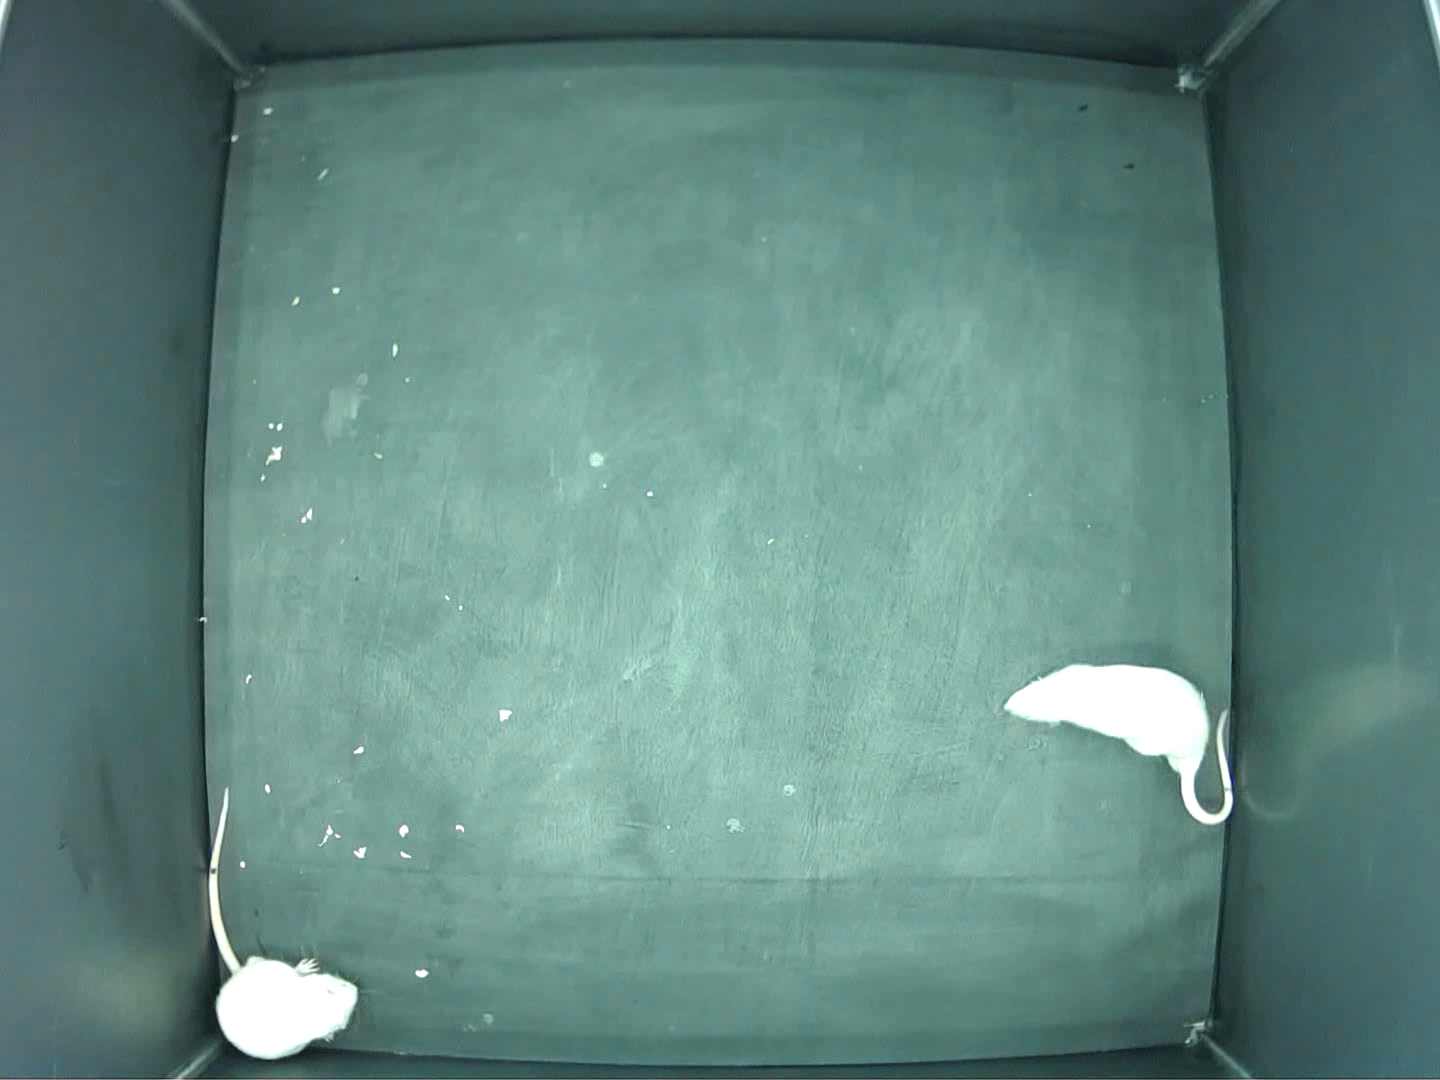
\includegraphics[width=0.27\linewidth]{images/ch02/action/turn/0964.png}
%   }
%   \subfigure[$t_0+2233~ms$]{\label{figure_turn_1302}
%   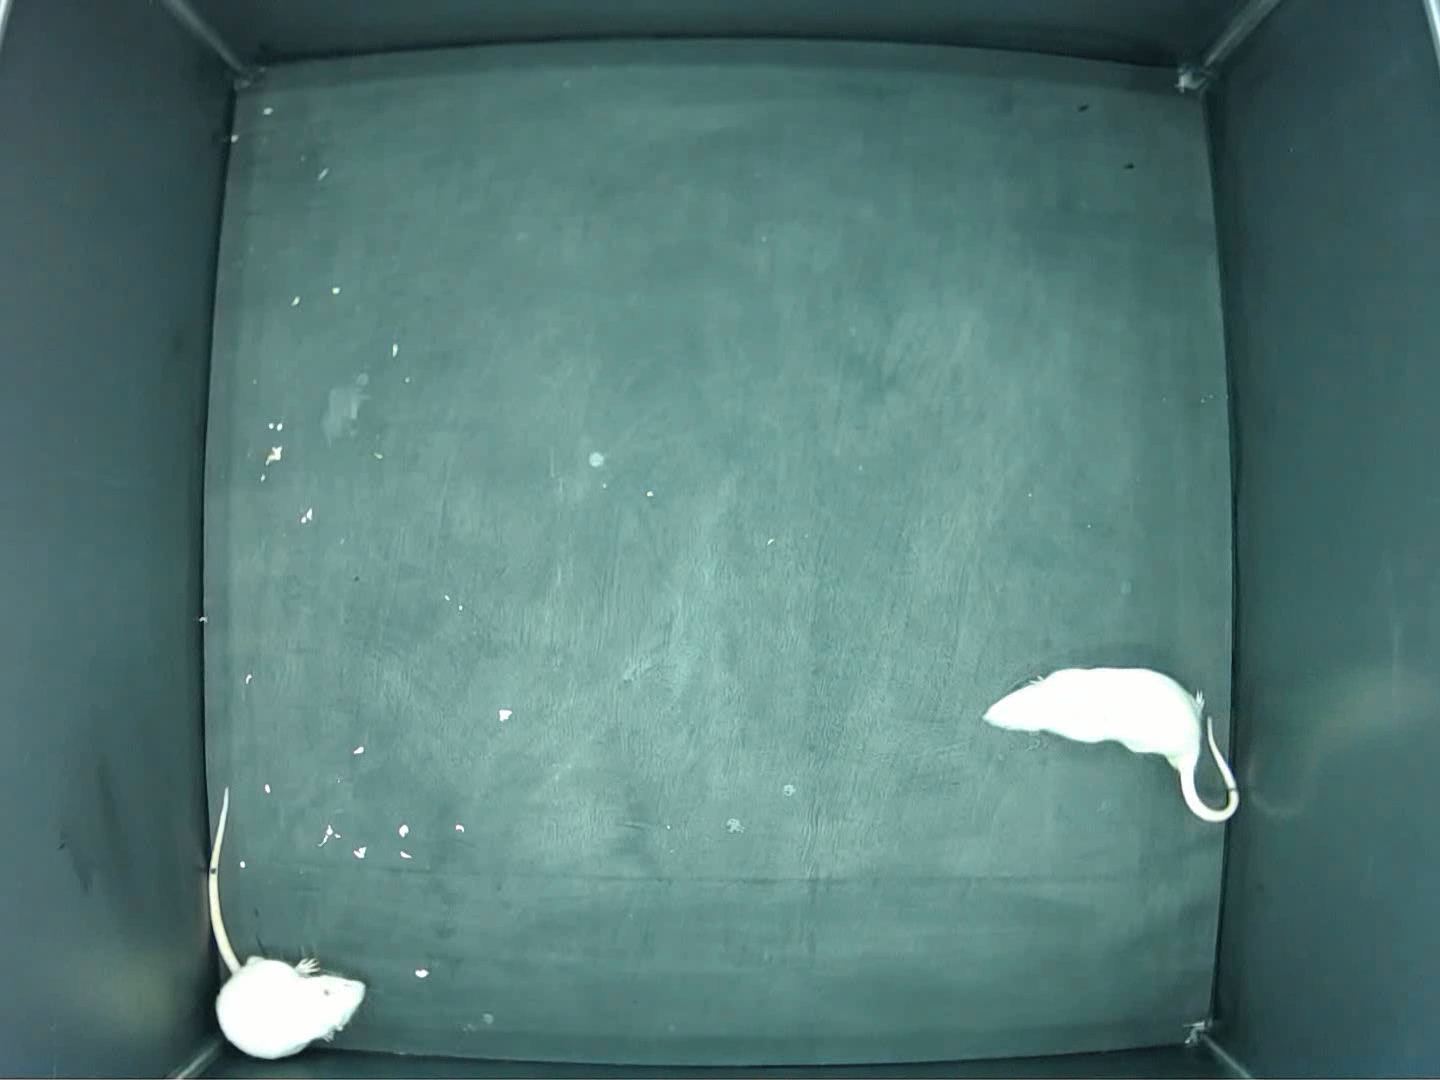
\includegraphics[width=0.27\linewidth]{images/ch02/action/turn/1302.png}
%   }
%   \subfigure[$t_0+2233~ms$]{\label{figure_turn_1650}
%   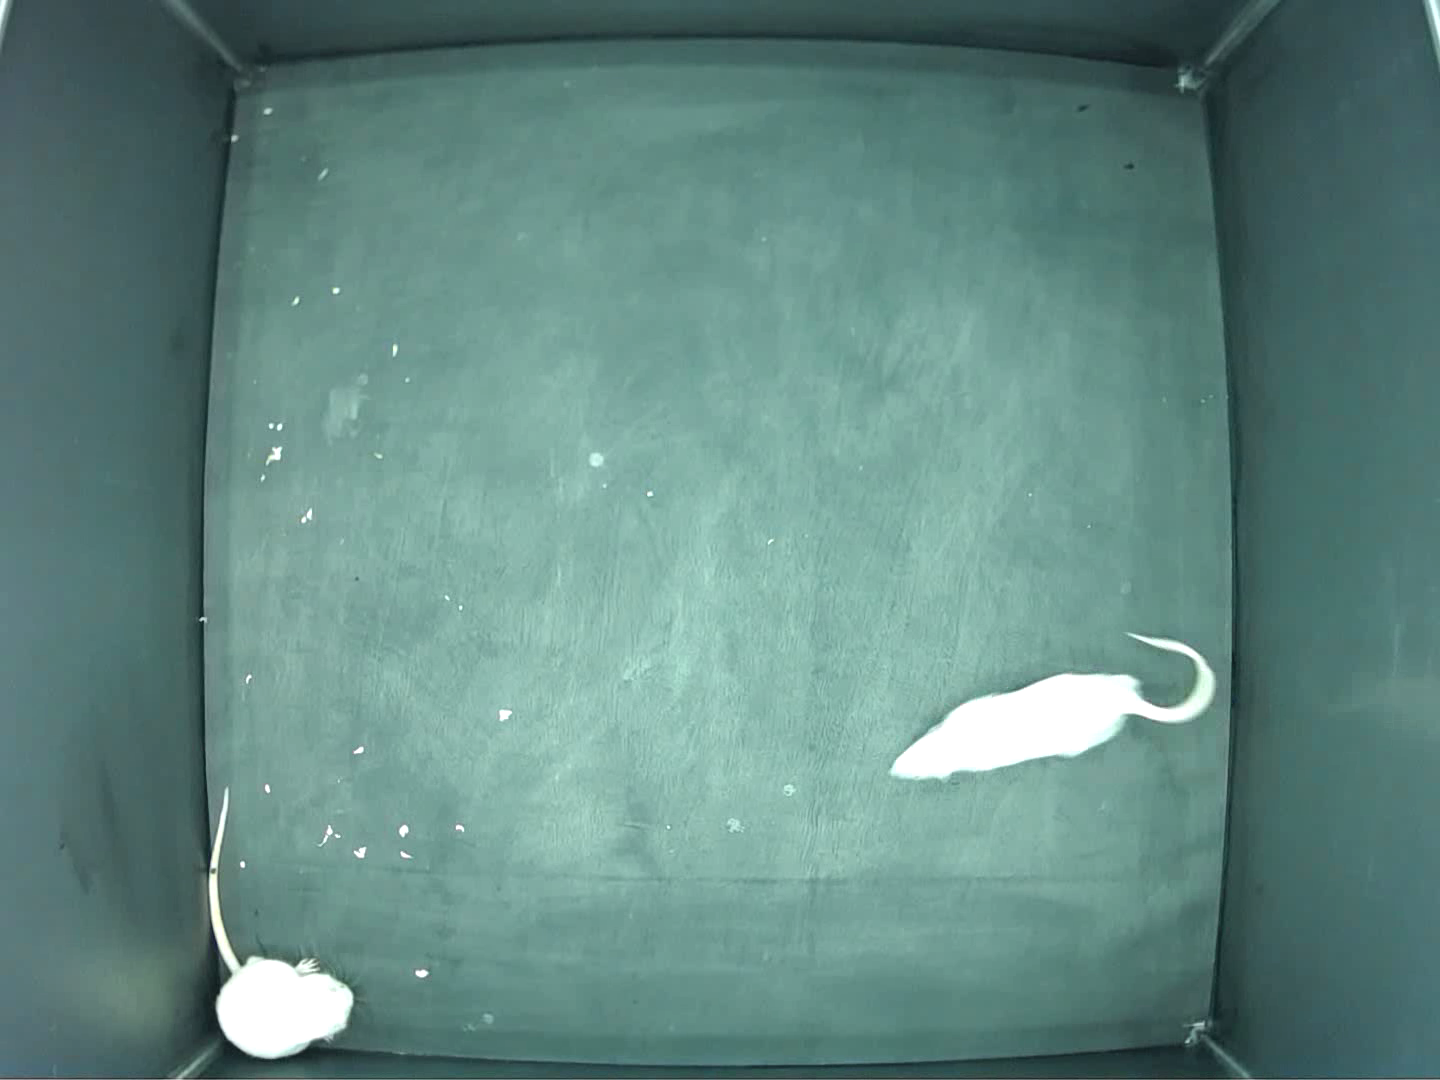
\includegraphics[width=0.27\linewidth]{images/ch02/action/turn/1650.png}
%   }
%   \caption{实验环境中生物鼠(右)左转}\label{figure_turn}
% \end{figure}
%     \item 直立是指生物鼠前肢离开地面,腰部与前身与地面构成一定夹角的动作(图\ref{rat_some}\subref{figure_rear})。在实验环境种,这一动作通常发生在生物鼠靠近墙壁时,因其前肢需要墙壁支撑以保持身体平衡。\label{pose_begin}
% %\begin{figure}[htbp]
% %  \vspace{13pt}
% %  \centering
% %  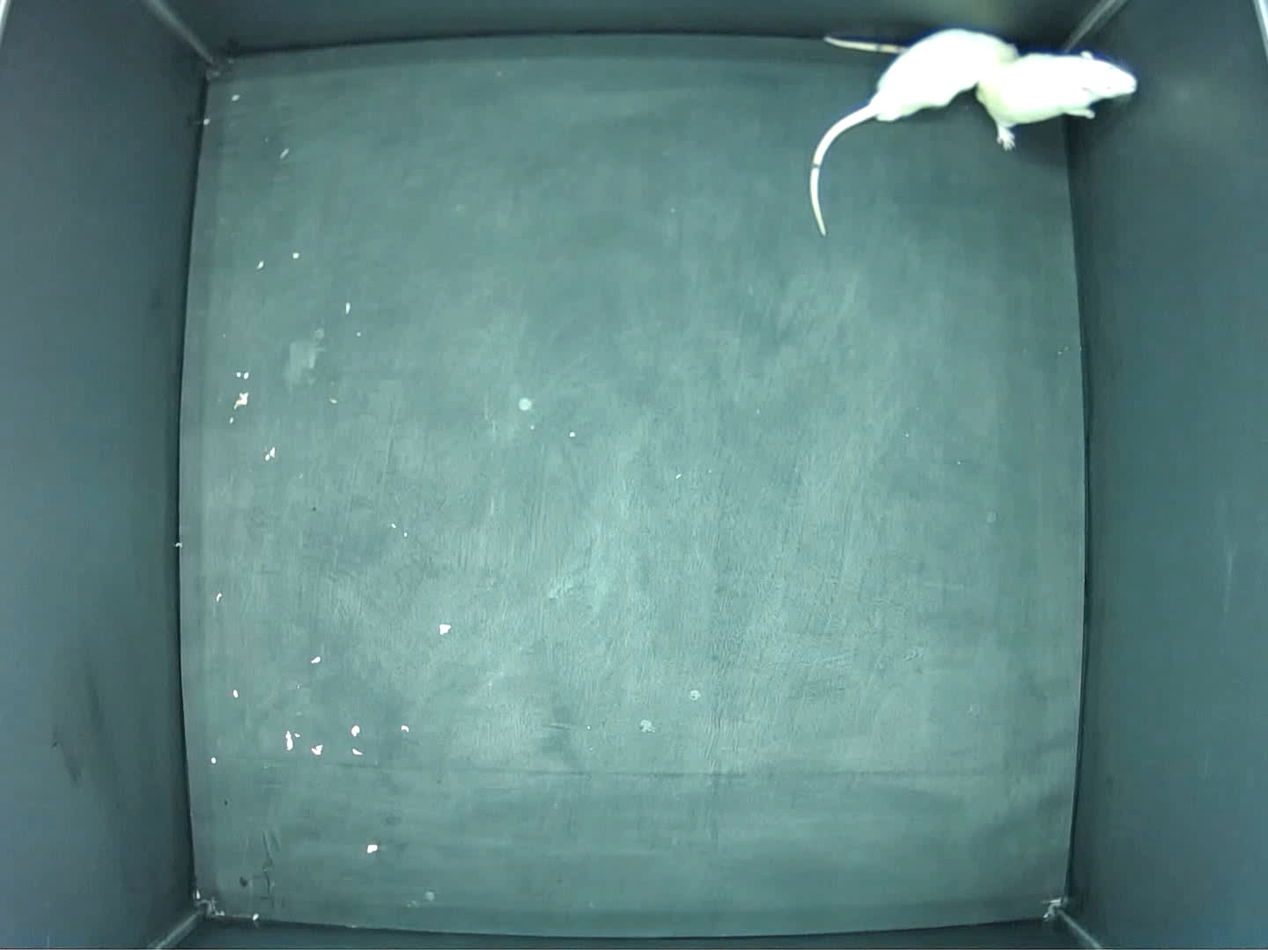
\includegraphics[width=0.4\linewidth]{images/ch02/action/rear.png}
% %  \caption{生物鼠(右)直立动作}\label{figure_rear}
% %\end{figure}

%         直立动作主要依靠其躯干各部分的协调。虽然生物鼠直立动作的起点存在差异,但其直立终点具有高度的相似性。因此,可以将机器鼠当前所处的任意状态作为执行治理动作的初始状态,设定固定的姿态作为完成直立动作的状态。通过相应的机械臂路径规划和插值算法等实现其躯干部分的平滑运动。
%     \item 嗅探(图\ref{figure_02_sniff})是生物鼠最常表现的动作之一,这是由于嗅觉是其主要的感觉途径之一\cite{whishawBehaviorLaboratoryRat2005}。在与其他生物鼠交互时,需要依靠气味辨别对方的特征;在觅食过程中,生物鼠依靠嗅探能够获得食物位置的部分信息;在探索时,生物鼠依赖嗅觉帮助确定环境的安全性。
% \begin{figure}[htbp]
%   %\vspace{13pt}
%   \centering
%   \subfigure[$t_0$]{\label{figure_sniff_0000}
%   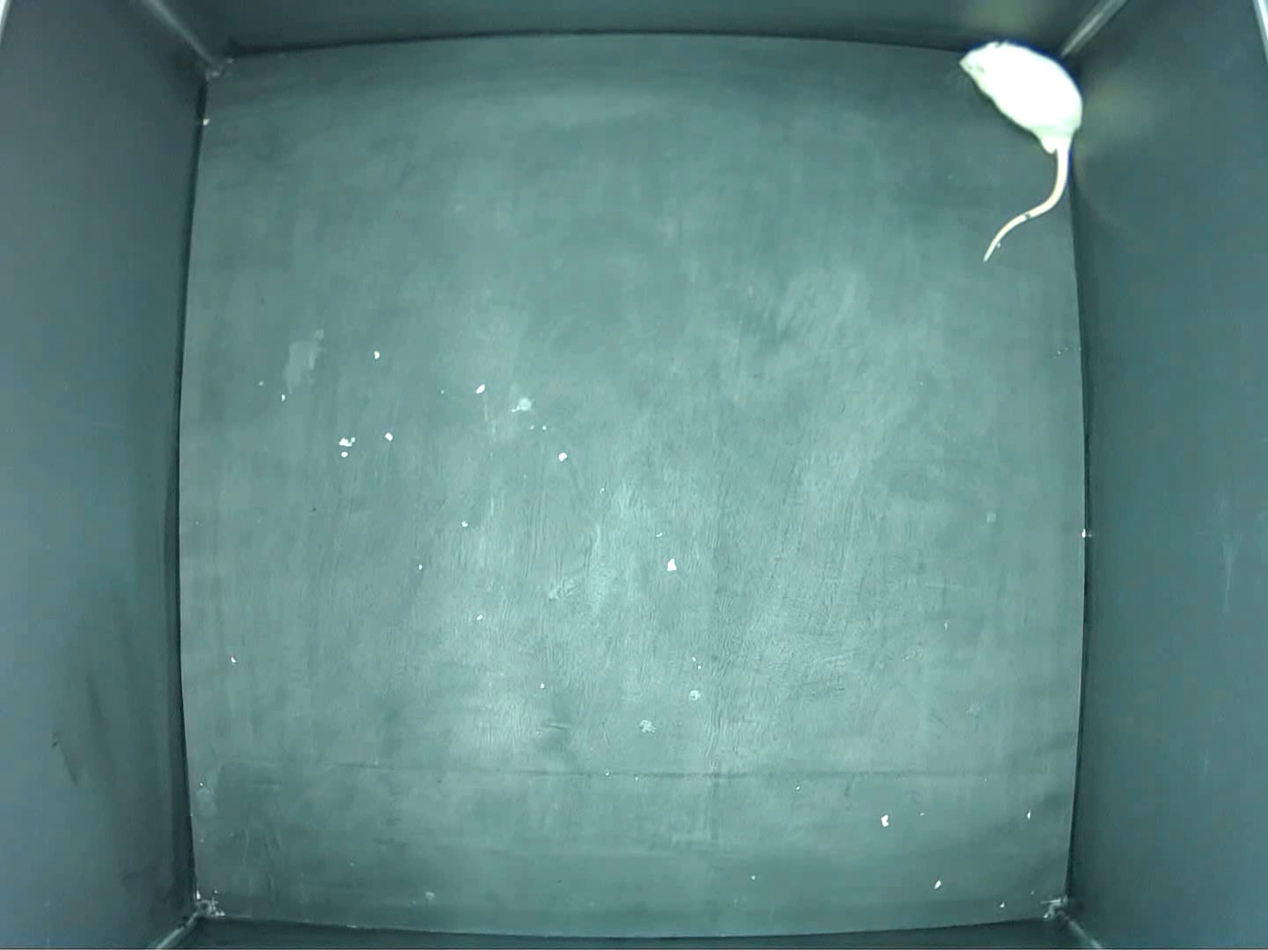
\includegraphics[height=0.23\linewidth]{images/ch02/action/sniff/000.png}
%   }
%   \subfigure[$t_0+344~ms$]{\label{figure_sniff_0430}
%   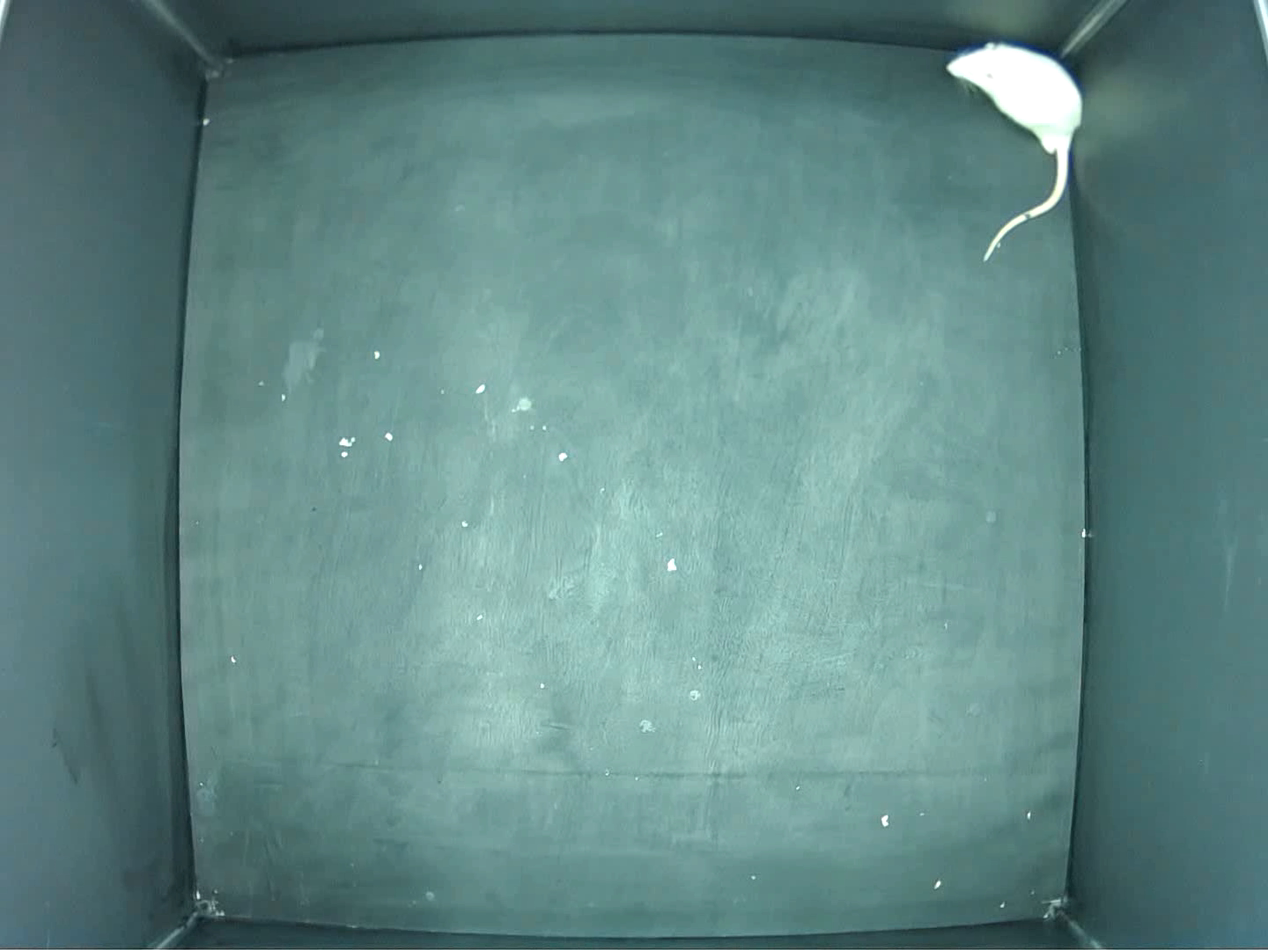
\includegraphics[height=0.23\linewidth]{images/ch02/action/sniff/344.png}
%   }
%   \subfigure[$t_0+752~ms$]{\label{figure_sniff_1050}
%   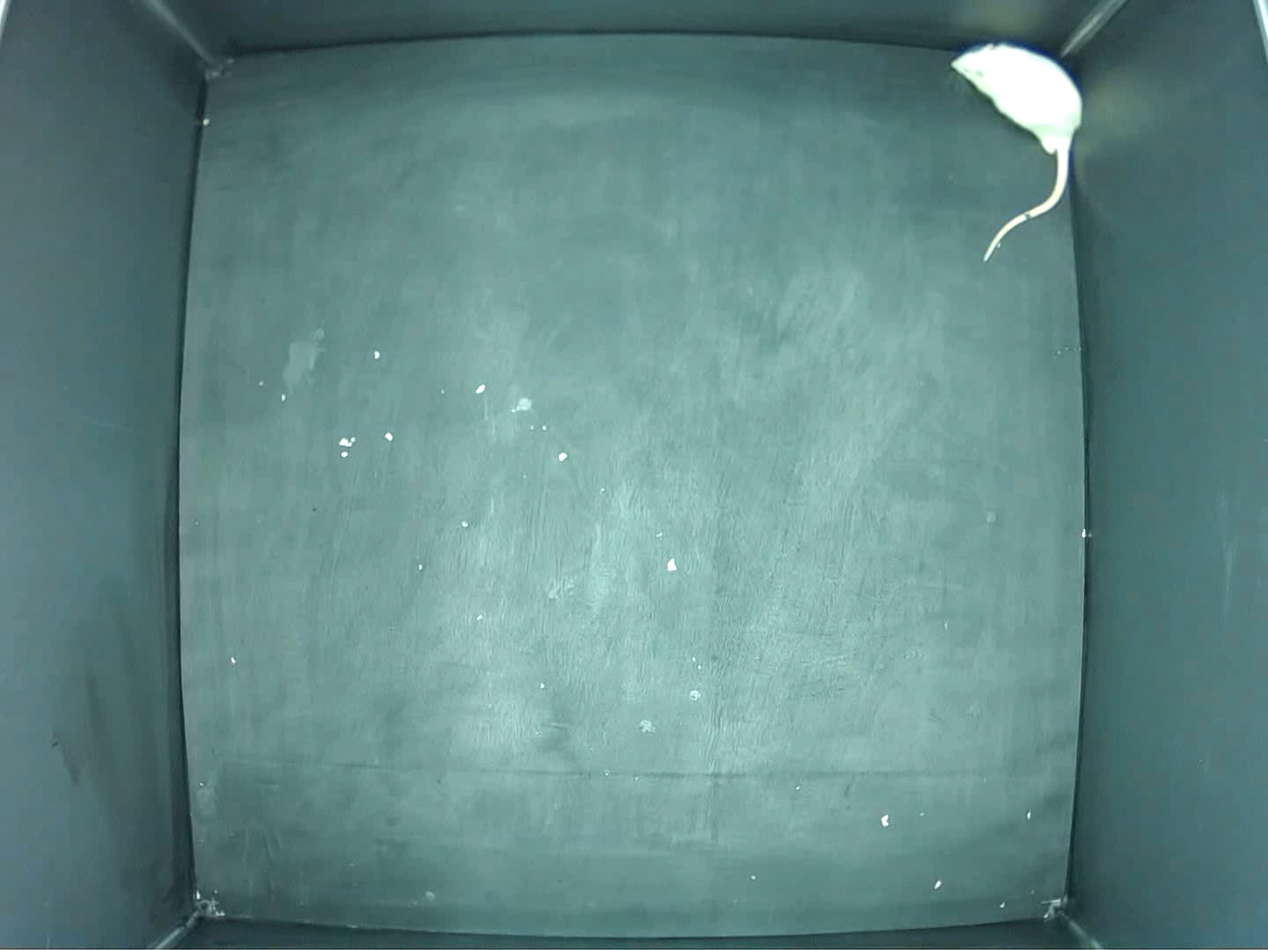
\includegraphics[height=0.23\linewidth]{images/ch02/action/sniff/752.png}
%   }
%   \caption{实验环境中生物鼠嗅探动作,头部有微小摆动}\label{figure_02_sniff}
% \end{figure}

%         在执行嗅探动作时,机器鼠的躯干部分应当处于较低位置,使其头部与地面或其他物体距离较近,便于嗅探。此外,嗅探动作的主要特点为头部的高频摆动,这可以依靠对机器鼠相应关节的单独控制实现。

%     \item 梳理是指对其交互伙伴皮肤区域的轻微撕咬的动作\cite{BarnettSTheRat}。这一行为通常被认为具有一定的攻击性,并且时常发生于领域内出现新的同类生物时。被梳理的动作与其对应,一般是领域内的“新来者”对已有生物鼠的臣服表现,而这种表现并不强烈。这一对动作表现如图\ref{rat_some}\subref{figure_groom&allow}。
% %\begin{figure}[htbp]
% %  \vspace{13pt}
% %  \centering
% %  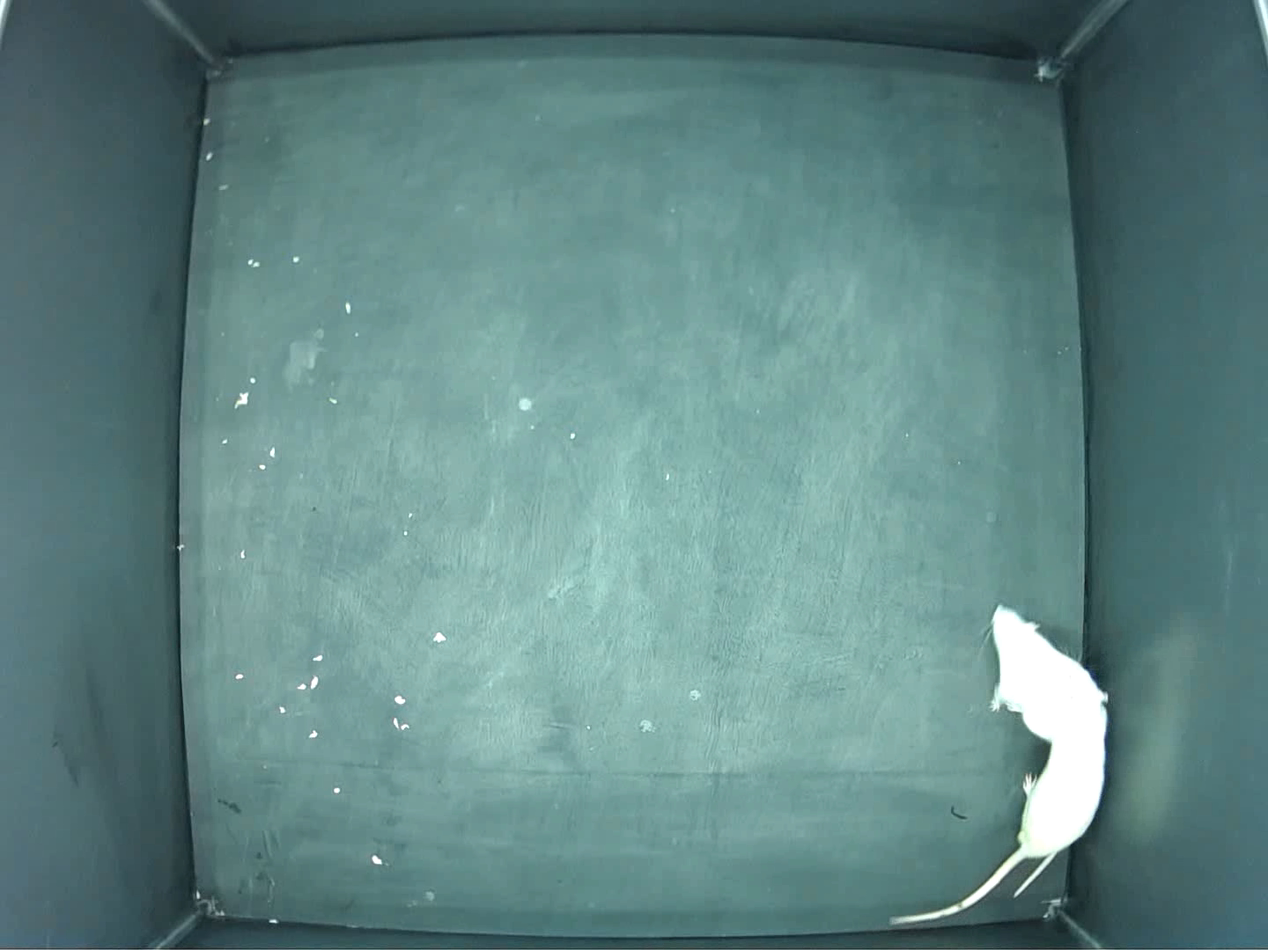
\includegraphics[width=0.4\linewidth]{images/ch02/action/groom&allow.png}
% %  \caption{生物鼠梳理与被梳理}\label{figure_groom&allow}
% %\end{figure}

%         实现对皮肤的撕咬需要保证机器鼠头部高度与交互伙伴身体高度相适应。
%     \item 与梳理和被梳理类似,攀爬和匍匐(图\ref{rat_some}\subref{figure_under&up})是另一对生物鼠交互的典型动作,不过与梳理相比,机器鼠“攀爬”时,头部和前肢置于另一生物鼠之上,具有更强的攻击性,这一对动作代表了生物鼠群内部一定的等级特征\cite{whishawBehaviorLaboratoryRat2005}。\label{pose_end}
% \begin{figure}[htbp]
%   %\vspace{13pt}
%   \centering
%   \subfigure[生物鼠(右)直立动作]{\label{figure_rear}
%   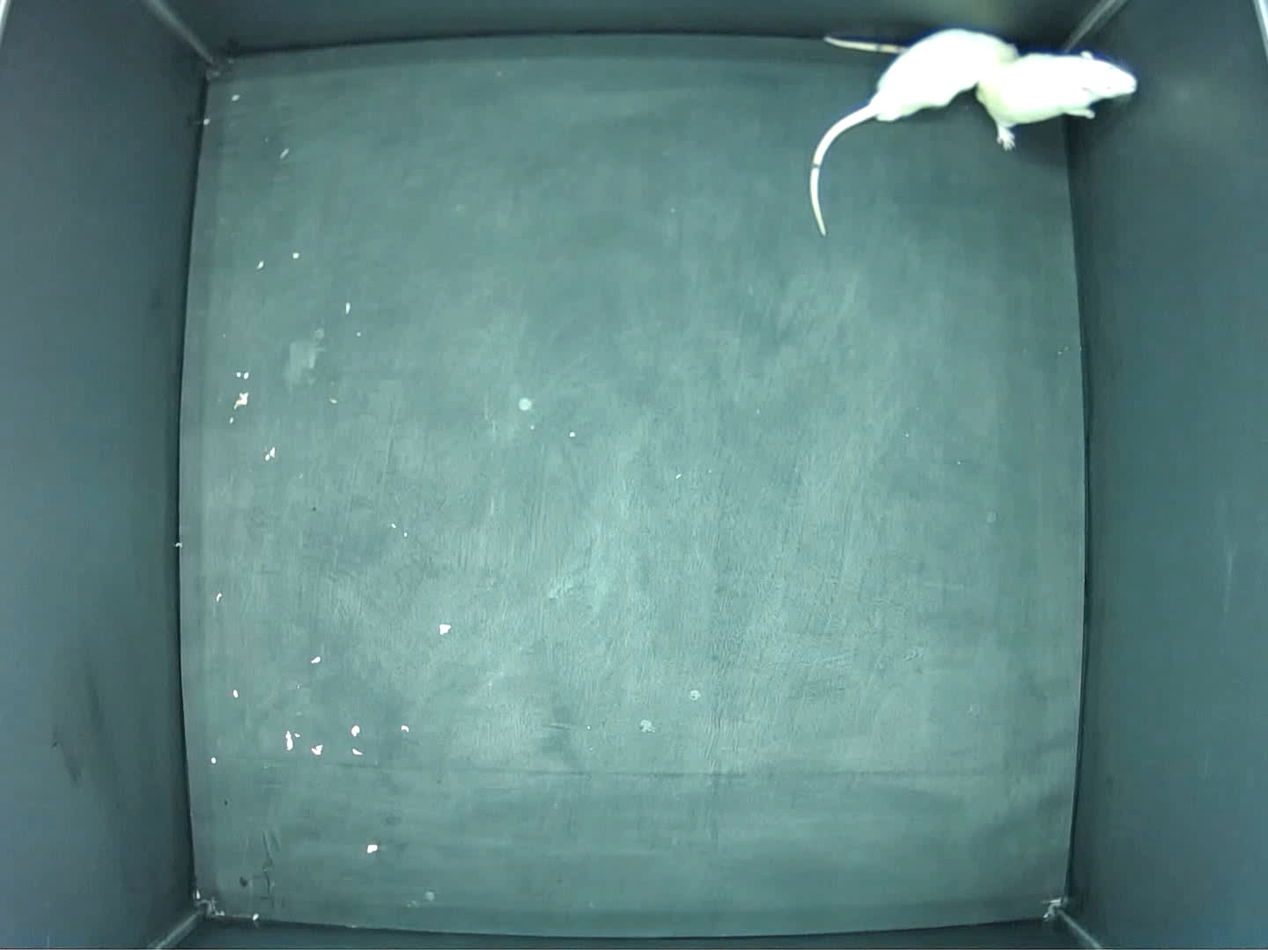
\includegraphics[width=0.27\linewidth]{images/ch02/action/rear.png}
%   }
%   \subfigure[梳理与被梳理]{\label{figure_groom&allow}
%   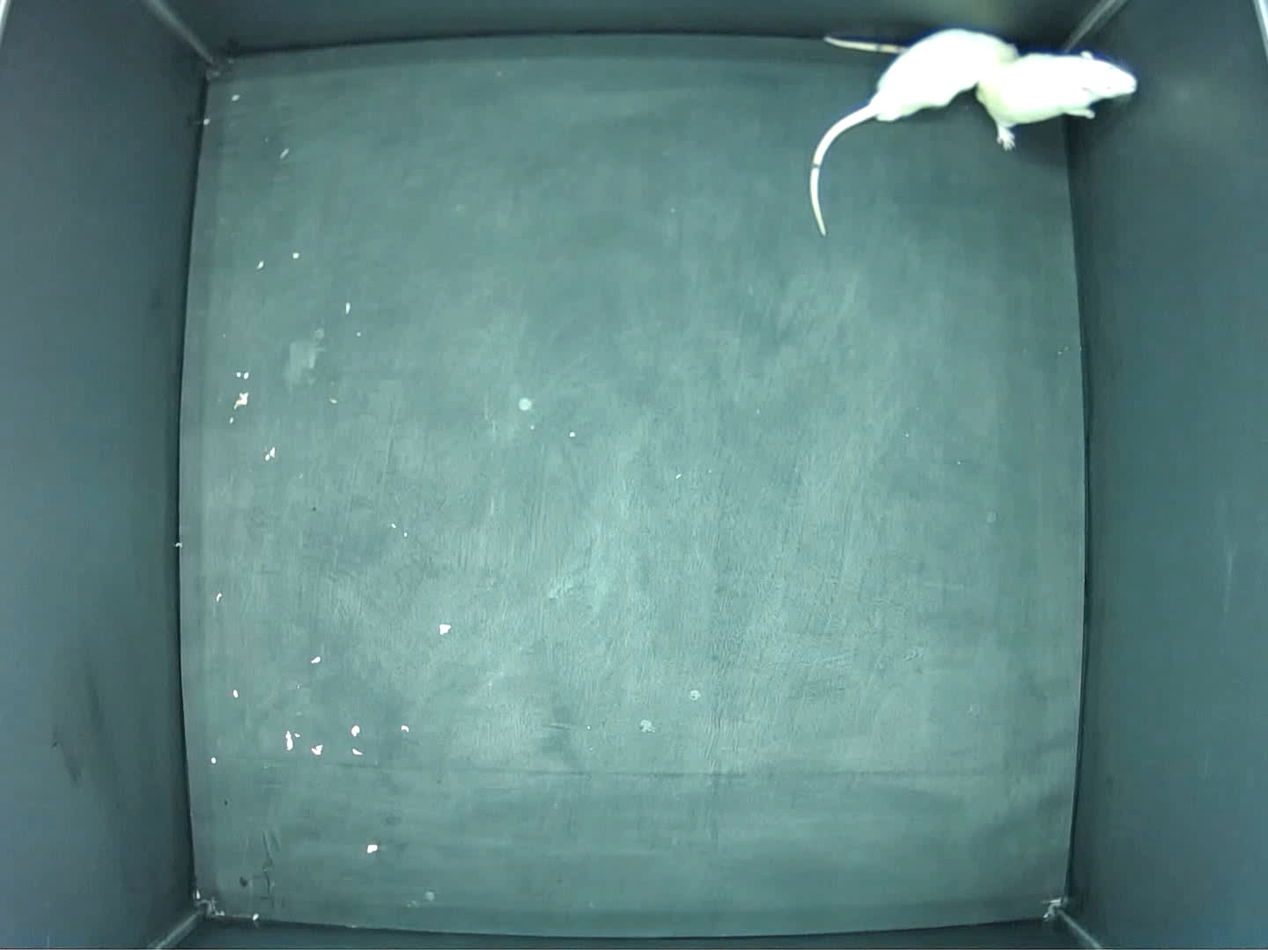
\includegraphics[width=0.27\linewidth]{images/ch02/action/rear.png}
%   }
%   \subfigure[攀爬和匍匐]{\label{figure_under&up}
%   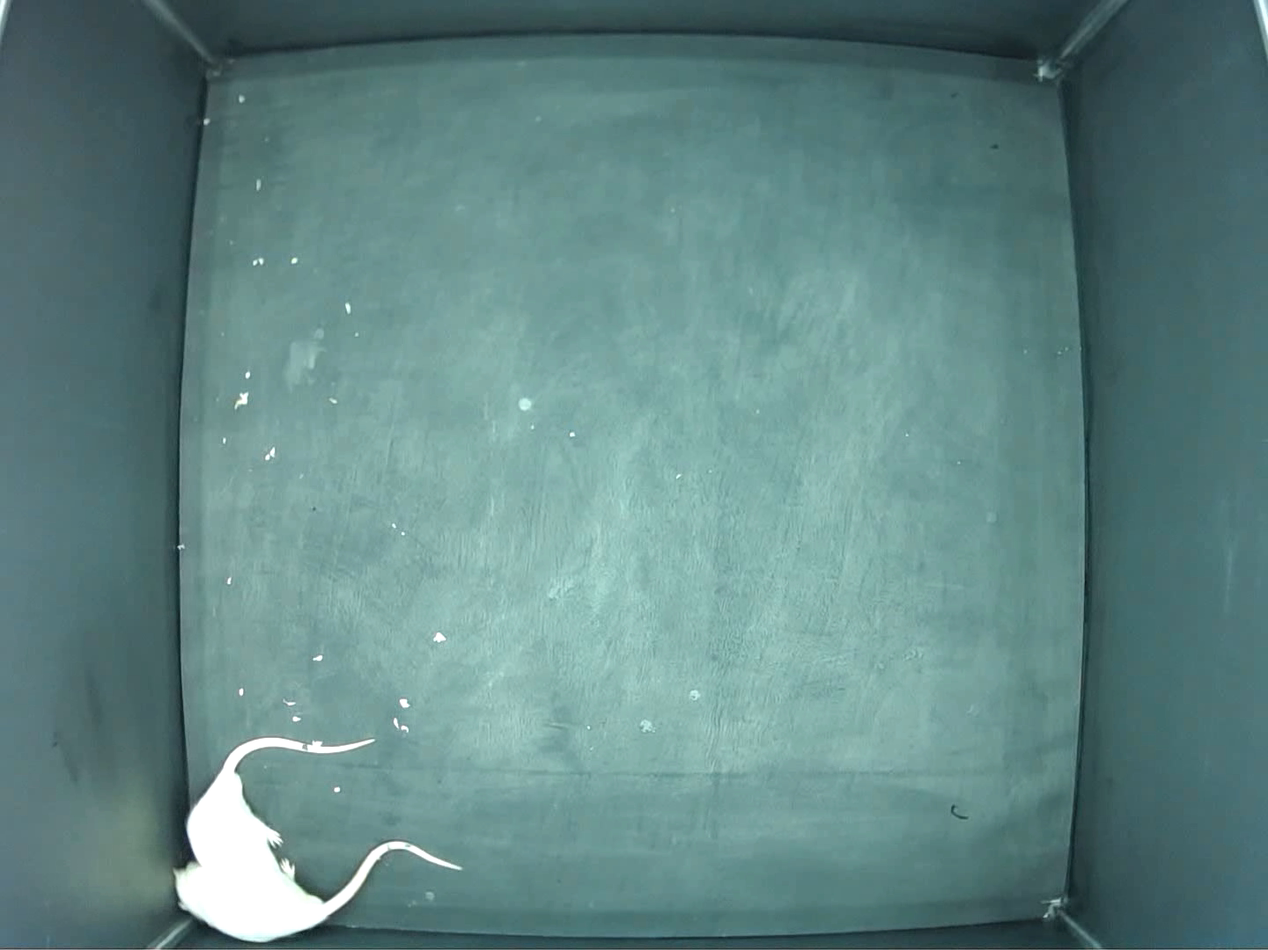
\includegraphics[width=0.27\linewidth]{images/ch02/action/under&up.png}
%   }
%   \caption{生物鼠执行部分动作时的姿态}\label{rat_some}
% \end{figure}
% \end{enumerate}

%         实现攀爬和匍匐时,需要考虑交互伙伴的相对位置,准确地将自身的前身置于合适的姿态。

% 上述\ref{pose_begin}\textasciitilde \ref{pose_end}动作均只涉及机器鼠躯干部分的关节位置变化,不同动作的最终状态关节位置如表\ref{table_jointpos}所示。
% \begin{table}[htbp]
%   \linespread{1.5}
%   \zihao{5}
%   \centering
%   \caption{机器鼠不同动作时关节位置表}\label{table_jointpos}
%   \begin{tabular}{*{8}{>{\centering\arraybackslash}p{1.5cm}}}
%     \toprule
%     动作                                       & $\theta_{1}(rad)$ & $\theta_{2}(rad)$ & $\theta_{3}(rad)$ & $\theta_{4}(rad)$  & $\theta_{5}(rad)$ & $\theta_{6}(rad)$ & $\theta_{7}(rad)$\\ \midrule
%     直立 & -0.8 & -0.2 & 0 & 0 & -0.2 & 0 & 0 \\
%     嗅探 & -0.1 & 0.15 & 0 & 0 & 0.15 & 0 & 0.15 \\
%     梳理 & -1 & 0.4 & -0.4 & -0.4 & 0.4 & 0.2 & 0.8 \\
%     被梳理 & -0.1 & 0.1 & -0.25 & -0.25 & 0.1 & 0.2 & 0.5 \\
%     攀爬 & -0.6 & 0.5 & 0 & 0 & 0.5 & 0 & 0.4 \\
%     匍匐 & 0 & -0.12 & 0 & 0 & -0.12 & 0 & -0.25 \\
%     \bottomrule
%     \end{tabular}
% \end{table}
